\documentclass[a4paper,11pt,oneside, titlepage]{article}
\usepackage[a4paper]{geometry} 
\geometry{a4paper,left=20mm, right=25mm, top=20mm, bottom=30mm} 
\usepackage[ngerman]{babel}
\usepackage{hyperref}
\usepackage{graphicx}
\usepackage[utf8x]{inputenc}
\usepackage[T1]{fontenc}
\usepackage{fancyhdr}
\usepackage{color}

\pagestyle{fancy}

\lhead{\today}
\chead{Gruppe: na17b}
\title{Handbuch für die Software: Nachrichtenkommunikation für das THW}
\author{na17b}
\date{}

\begin{document}
	\maketitle
	\pagenumbering{gobble}
	\tableofcontents
	
	\newpage
	\pagenumbering{arabic}
	
	\section{Landing Page}
	Lädt man die Anwendung neu so befindet man sich auf der Landing Page. Auf dieser werden sämtliche notwendigen Login Daten erfragt.
	\newline
	Mithilfe von \glqq{}Felder leeren\grqq{} können alle Eingaben und Wahlen zurückgesetzt werden inklusive des ggf. bereits ausgewählten Einsatzes.
	Mit \glqq{}Eingaben speichern\grqq{} werden die eingegeben Daten bestätigt.
	
	\subsection{Rollenauswahl}
	Bei dieser werden verschiedene Rollen aufgelistet. Zu jeder wird der Absendername und das Handzeichen erfragt, wobei bei der Rolle Sachgebietsleiter (SGL) noch das dazugehörige Sachgebiet angegeben werden muss.
	
	\subsection{Einsätze}
	Unter der Rollenauswahl befindet sich die Auswahl des Einsatzes.
	Muss ein neuer Einsatz angelegt werden, so ist das über den Button \glqq{}Einsatz erstellen\grqq{} möglich. Es klappen sich Eingabefelder für die benötigten Daten auf, die sich aus Einsatznamen, Einsatzadresse und der Art des Stabes zusammensetzen. Nach vollständigen Ausfüllen muss auf den Button \glqq{} Einsatz speichern \grqq{} geklickt werden, woraufhin er automatisch als aktueller Einsatz ausgewählt wird. Des Weiteren ist der erstellte Einsatz jetzt unter \glqq{} Einsatz auswählen \grqq zufinden.
	\newline
	\newline
	Klickt man auf den Button \glqq{}Einsatz auswählen\grqq{} so klappt eine Tabelle bereits vorhandener Einsätze mit den dazugehörigen Daten auf: Name, Adresse und Art des Stabes. Mit einem Klick auf den gesuchten Einsatz wählt man diesen aus.
	
	\begin{figure}[htpb]
		\centering
		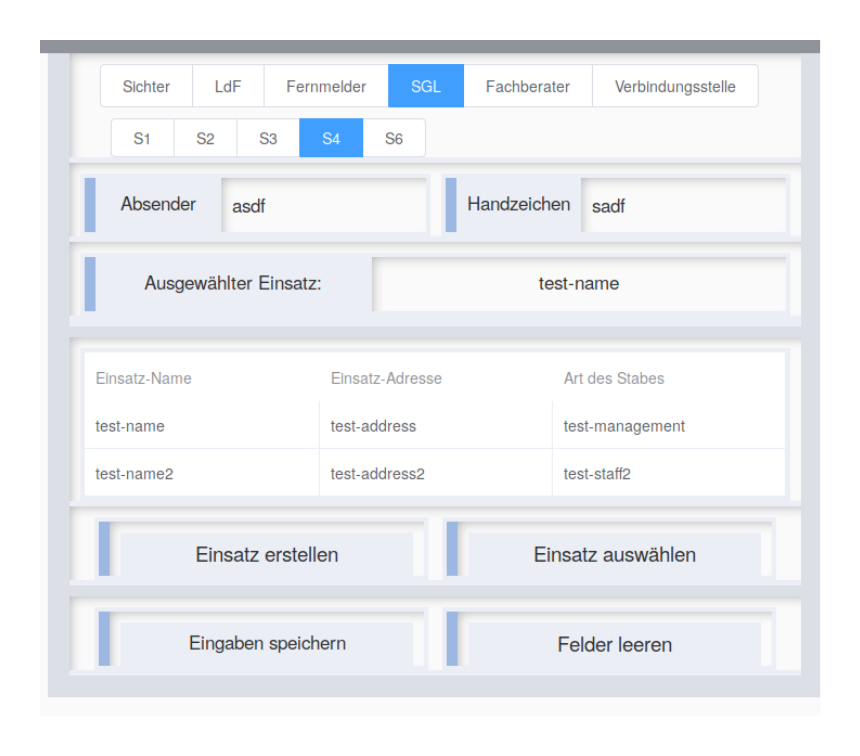
\includegraphics[width=0.8\linewidth]{lPage}
		\caption{Landing Page mit Beispiel Einsätzen}
	\end{figure}
	\newpage
	
	\section{Übersicht}
	Ist man eingeloggt so sieht man eine Übersichtsseite. Diese ist unterteilt in Header, zwei Sidebars und eine Mittelsektion.
	Der Header zeigt von links nach rechts einen Platzhalter für ein Logo und den Schriftzug \glqq{} Nachrichtenkom. für das THW\grqq{}, den aktuellen Einsatz, das auf der Landing Page eingetragene Handzeichen, ein rollenspezifisches Symbol und zu guter letzt die Rollenbezeichnung an. 
	Befindet man sich mit dem Mauszeiger über der Rollenbezeichnung, so eröffnet sich durch einen Klick auf genau diesen, die Funktion den Nutzer wechseln zu können. Dies wird durch die Veränderung des Cursors angezeigt.
		
	\section{Formularübersicht}
	Loggt man sich erstmals ein so wird man direkt auf die Formularübersicht weitergeleitet. Dort werden standardmäßig Formulare angezeigt, die zu bearbeiten sind, gefiltert nach der besetzten Rolle.
	Pro Formular wird eine Zeile mit den dazugehörigen Status, der Technischen Betriebsbuchnummer, Verfasser, Sichterkürzel, Datum, Uhrzeit, Empfänger und Kurzinhalt angezeigt. Zum Auswählen eines Formulares klickt man einfach auf das entsprechende. So wird das bis dorthin ausgefüllte angezeigt und kann bearbeitet werden.
	\newline
	\newline
	In der rechten Sidebar stehen Filteroptionen zur Verfügung. So befindet sich ganz oben ein Eingabefeld in dem nach beliebigen Zeichenfolgen für den Inhalt, der Technische Betriebsbuchnummer und eine Gegenstelle gesucht werden kann. Will man nach Sichter oder Verfasser suchen, so muss das vollständige und richtige Handzeichen eingegeben werden. Ebenfalls kann nach angelegten Einsätzen gefiltert werden, wobei standardmäßig nur Formulare des aktuellen angezeigt werden.
	\newline
	Weitere Filteroptionen sind unter \glqq{}Status \grqq{} in eingehende (\glqq{}Eingang\grqq{}) und ausgehende (\glqq{}Ausgang\grqq{}) untergliedert. Abbildung 2 und 3 dienen zur Veranschaulichung welche Rolle welche Status standardmäßig sieht. 

	\begin{figure}[htpb]

	\centering
	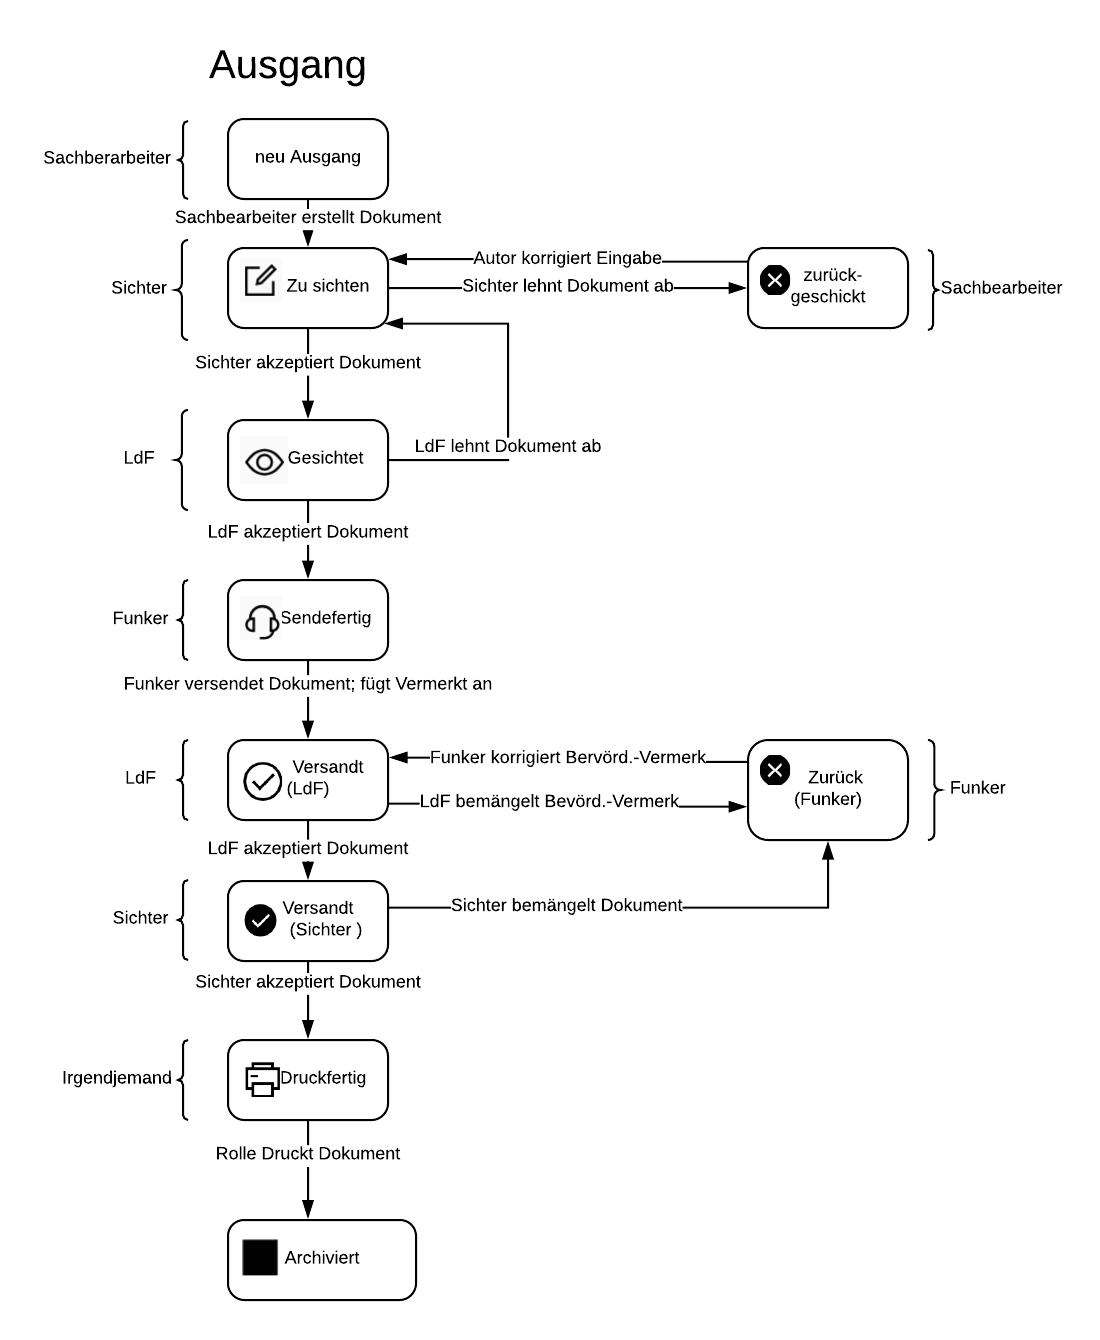
\includegraphics[width=0.8\linewidth]{HBausgang}
	\caption{}

	\end{figure}
	\newpage	
	\begin{figure}[htpb]
		\centering
		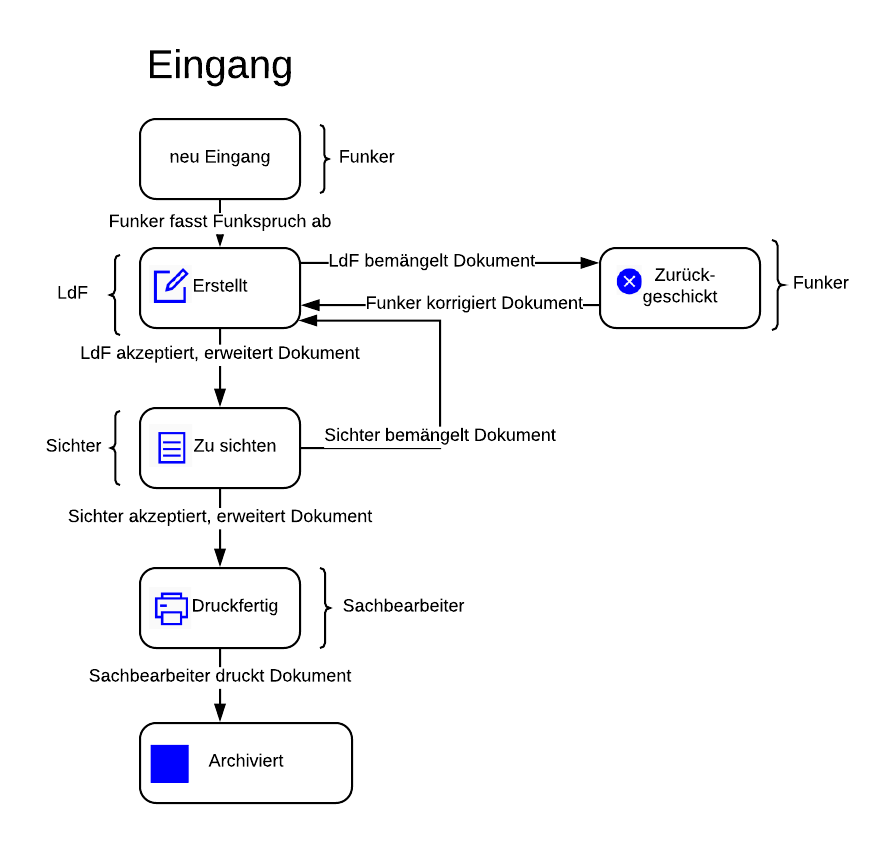
\includegraphics[width=0.8\linewidth]{HBeingang}
		\caption{}
	\end{figure}
	
	\section{Formulare}
	Genau wie der Vierfachvordruck kommen Formulare in vielen Farben und Formen. Für alle Formulare gibt es jedoch einheitliche Regelungen.
	\newline
	Im Normalfall sind nur die weiß hinterlegten Felder im auszufüllen. Es ist nicht vorgesehen die ausgegrauten Bereiche auszufüllen,jedoch für Sonderfälle möglich.
	\newline
	Des Weiteren steht in jedem Fall ein \glqq{} Zurücksetzten\grqq{} -Button zur Verfügung. Dieser setzt das vorliegende Formular immer auf den Stand zurück, auf dem es aufgerufen wurde.
	\newline
	Zu Beachten ist ebenfalls, dass Zeitangaben automatisch ausgefüllt werden, sobald man auf \glqq{} Abschicken \grqq{} drückt.
	
	\subsection{Neues Formular}
	Um ein neues Formular auszufüllen muss in der linken Sidebar auf den zweiten Button von oben geklickt werden. Daraufhin öffnet sich ein neues Unausgefülltes mit blauen Rand.
	\newline
	In der rechten Sidebar befinden sich die Buttons \glqq{}Abschicken\grqq{} und \glqq{}Zurücksetzen\grqq{}.
	Mithilfe des Zurücksetzen-Buttons wird das komplette Formular geleert. Sobald das Formular nach besten Gewissen ausgefüllt ist, kann durch \glqq{} Abschicken \grqq{} die Nachricht an den LdF versandt werden.
	\newline
	Wird die Seite ohne Absenden des Formulares verlassen, wird gefragt ob das Formular als Entwurf gespeichert werden solle.
	
	\subsection{andere Formulare}
	Formulare die von der Formularübersicht aufgerufen werden, haben eine spezifische Farbgebung und andere zur Verfügung stehenden Buttons. Um dies anschaulich darzustellen, wurde folgende Tabelle entworfen:
	
	\begin{figure}[htpb]
			
		\centering
		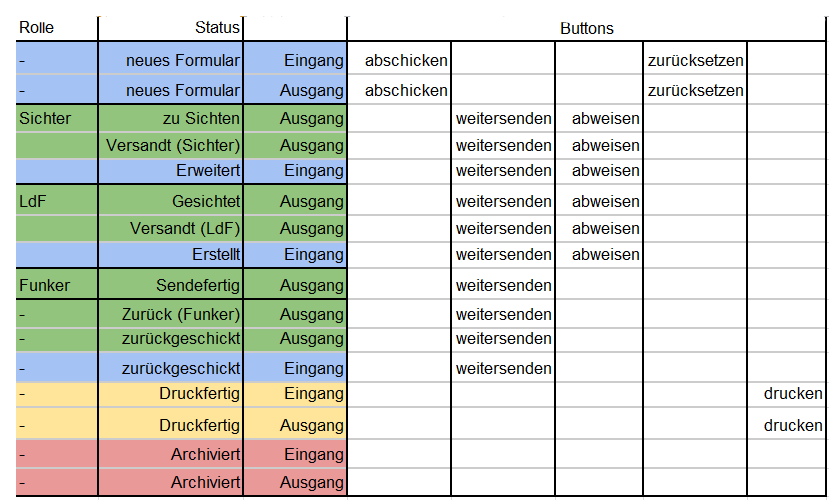
\includegraphics[width=0.8\linewidth]{sichten}
		\caption{Sichten der unterschiedlichen Rollen}
	
		\end{figure}
	
	
	\section{Entwurf}
	Wird diese Seite aufgerufen, so ist hier ein nicht versendetes Formular zu finden. In der rechten Sidebar stehen alle Optionen zur Verfügung, die beim erstmaligen Öffnen des Formulares auch vorhanden waren, sodass der Nachrichtenfluss gewährleistet ist.
	\newline
	Zu beachten ist, dass hier stets nur ein Entwurf gespeichert werden kann. 
	
\end{document}